\documentclass[tikz,border=8pt]{standalone}
\usepackage{xcolor}
\usepackage{tikz}
\usetikzlibrary{positioning,fit,backgrounds,arrows.meta,matrix}

% Tutorial palette
\definecolor{sqfill}{HTML}{ccccff}
\definecolor{sqstroke}{HTML}{000099}
\definecolor{ifill}{HTML}{7373ff}
\definecolor{istroke}{HTML}{0000cc}
\definecolor{newfill}{HTML}{ffbf80}
\definecolor{newstroke}{HTML}{cc6600}
\definecolor{boxfill}{HTML}{f5f5f5}
\definecolor{boxstroke}{HTML}{a6a6a6}

\tikzset{
  sq/.style={circle, fill=sqfill, draw=sqstroke, line width=0.8pt,
             minimum size=9pt, inner sep=0pt},
  sqI/.style={circle, fill=ifill, draw=istroke, line width=0.8pt,
              minimum size=9pt, inner sep=0pt},
  sqIL/.style={circle, fill=ifill, draw=istroke, line width=1pt,
               minimum size=14pt, inner sep=0pt, font=\tiny},
  newnode/.style={circle, fill=newfill, draw=newstroke, line width=1pt,
                  minimum size=14pt, inner sep=0pt, font=\tiny},
  acsbox/.style={draw=boxstroke, fill=boxfill, rounded corners=3pt,
                 inner sep=5pt},
  morpharrow/.style={-{Latex[length=4pt,width=3pt]}, thin},
  spanarrow/.style={-{Latex[length=5pt,width=3.5pt]}, thick,
                    shorten <=5pt, shorten >=5pt},
  matcharrow/.style={-{Latex[length=5pt,width=3.5pt]}, thick,
                     shorten <=5pt, shorten >=5pt}
}

% DPO rewrite for mark_x on a 3x3 TicTacToe board
%
%   L <-l- K -r-> R
%   |       |      |
%   m       k      m'
%   v       v      v
%   G <-g- D -g'-> G'
%
% L = K = one Sq (the empty square to mark)
% R = Sq + X piece (xsq morphism)
% G, D = 3x3 board with center matched (D = G since l = identity)
% G' = board after placing X at center
\begin{document}
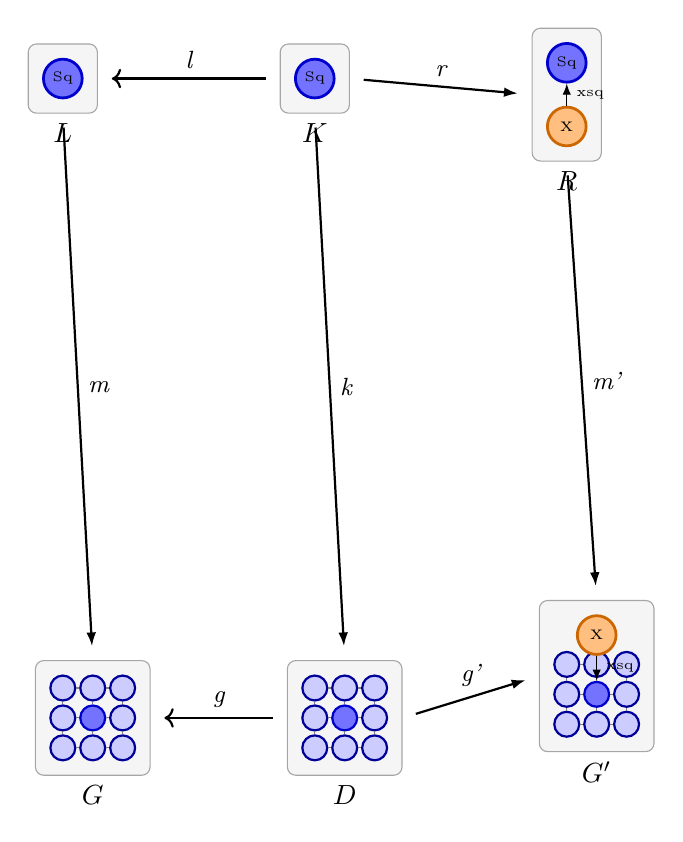
\begin{tikzpicture}

  % ===== Top row: L, K, R =====

  % L: one interface Sq
  \node[sqIL] (L-sq) at (0, 8.5) {Sq};
  \begin{pgfonlayer}{background}
    \node[acsbox, fit=(L-sq), label={[font=\itshape]below:$L$}] (Lbox) {};
  \end{pgfonlayer}

  % K: one interface Sq
  \node[sqIL] (K-sq) at (3.2, 8.5) {Sq};
  \begin{pgfonlayer}{background}
    \node[acsbox, fit=(K-sq), label={[font=\itshape]below:$K$}] (Kbox) {};
  \end{pgfonlayer}

  % R: interface Sq + new X
  \node[sqIL]  (R-sq) at (6.4, 8.7) {Sq};
  \node[newnode, below=8pt of R-sq] (R-x) {X};
  \draw[morpharrow] (R-x) -- node[right, font=\tiny]{xsq} (R-sq);
  \begin{pgfonlayer}{background}
    \node[acsbox, fit=(R-sq)(R-x), label={[font=\itshape]below:$R$}] (Rbox) {};
  \end{pgfonlayer}

  % Top row span arrows
  \draw[spanarrow, <-] (Lbox.east) -- node[above, font=\small\itshape]{l} (Kbox.west);
  \draw[spanarrow]     (Kbox.east) -- node[above, font=\small\itshape]{r} (Rbox.west);

  % ===== Bottom row: G, D, G' (3x3 boards) =====
  % Grid spacing: 0.38cm per cell
  \def\gs{0.38}  % grid step

  % --- G board (center Sq is matched = interface color) ---
  \foreach \r in {0,1,2} {
    \foreach \c in {0,1,2} {
      \pgfmathsetmacro{\px}{\c*\gs}
      \pgfmathsetmacro{\py}{\r*\gs}
      \ifnum\r=1\ifnum\c=1
        \node[sqI] (G-\r-\c) at (\px, \py) {};
      \else
        \node[sq]  (G-\r-\c) at (\px, \py) {};
      \fi\else
        \node[sq]  (G-\r-\c) at (\px, \py) {};
      \fi
    }
  }
  % Row edges (horizontal gray lines)
  \foreach \r in {0,1,2} {
    \foreach \c in {0,1} {
      \pgfmathtruncatemacro{\cnext}{\c+1}
      \draw[gray, thin] (G-\r-\c) -- (G-\r-\cnext);
    }
  }
  % Col edges (vertical gray lines)
  \foreach \c in {0,1,2} {
    \foreach \r in {0,1} {
      \pgfmathtruncatemacro{\rnext}{\r+1}
      \draw[gray, thin] (G-\r-\c) -- (G-\rnext-\c);
    }
  }
  \begin{pgfonlayer}{background}
    \node[acsbox, fit=(G-0-0)(G-2-2), label={[font=\itshape]below:$G$}] (Gbox) {};
  \end{pgfonlayer}

  % --- D board (identical to G: l = identity, nothing deleted) ---
  \foreach \r in {0,1,2} {
    \foreach \c in {0,1,2} {
      \pgfmathsetmacro{\px}{3.2 + \c*\gs}
      \pgfmathsetmacro{\py}{\r*\gs}
      \ifnum\r=1\ifnum\c=1
        \node[sqI] (D-\r-\c) at (\px, \py) {};
      \else
        \node[sq]  (D-\r-\c) at (\px, \py) {};
      \fi\else
        \node[sq]  (D-\r-\c) at (\px, \py) {};
      \fi
    }
  }
  \foreach \r in {0,1,2} {
    \foreach \c in {0,1} {
      \pgfmathtruncatemacro{\cnext}{\c+1}
      \draw[gray, thin] (D-\r-\c) -- (D-\r-\cnext);
    }
  }
  \foreach \c in {0,1,2} {
    \foreach \r in {0,1} {
      \pgfmathtruncatemacro{\rnext}{\r+1}
      \draw[gray, thin] (D-\r-\c) -- (D-\rnext-\c);
    }
  }
  \begin{pgfonlayer}{background}
    \node[acsbox, fit=(D-0-0)(D-2-2), label={[font=\itshape]below:$D$}] (Dbox) {};
  \end{pgfonlayer}

  % --- G' board (center Sq + new X piece) ---
  \foreach \r in {0,1,2} {
    \foreach \c in {0,1,2} {
      \pgfmathsetmacro{\px}{6.4 + \c*\gs}
      \pgfmathsetmacro{\py}{\r*\gs + 0.3}
      \ifnum\r=1\ifnum\c=1
        \node[sqI] (Gp-\r-\c) at (\px, \py) {};
      \else
        \node[sq]  (Gp-\r-\c) at (\px, \py) {};
      \fi\else
        \node[sq]  (Gp-\r-\c) at (\px, \py) {};
      \fi
    }
  }
  \foreach \r in {0,1,2} {
    \foreach \c in {0,1} {
      \pgfmathtruncatemacro{\cnext}{\c+1}
      \draw[gray, thin] (Gp-\r-\c) -- (Gp-\r-\cnext);
    }
  }
  \foreach \c in {0,1,2} {
    \foreach \r in {0,1} {
      \pgfmathtruncatemacro{\rnext}{\r+1}
      \draw[gray, thin] (Gp-\r-\c) -- (Gp-\rnext-\c);
    }
  }
  % New X piece at center
  \node[newnode, above=9pt of Gp-1-1] (Gp-x) {X};
  \draw[morpharrow] (Gp-x) -- node[right, font=\tiny]{xsq} (Gp-1-1);
  \begin{pgfonlayer}{background}
    \node[acsbox, fit=(Gp-0-0)(Gp-2-2)(Gp-x),
          label={[font=\itshape]below:$G'$}] (Gpbox) {};
  \end{pgfonlayer}

  % ===== Vertical match arrows =====
  \draw[matcharrow] (Lbox.south) -- node[right, font=\small\itshape]{m}  (Gbox.north);
  \draw[matcharrow] (Kbox.south) -- node[right, font=\small\itshape]{k}  (Dbox.north);
  \draw[matcharrow] (Rbox.south) -- node[right, font=\small\itshape]{m'} (Gpbox.north);

  % ===== Bottom horizontal arrows =====
  \draw[spanarrow, <-] (Gbox.east) -- node[above, font=\small\itshape]{g}   (Dbox.west);
  \draw[spanarrow]     (Dbox.east) -- node[above, font=\small\itshape]{g'}  (Gpbox.west);

\end{tikzpicture}
\end{document}
